\documentclass[dvipsnames]{article}
\usepackage{xcolor}
\usepackage{chemfig}
\begin{document}
\thispagestyle{empty}
\begin{figure}
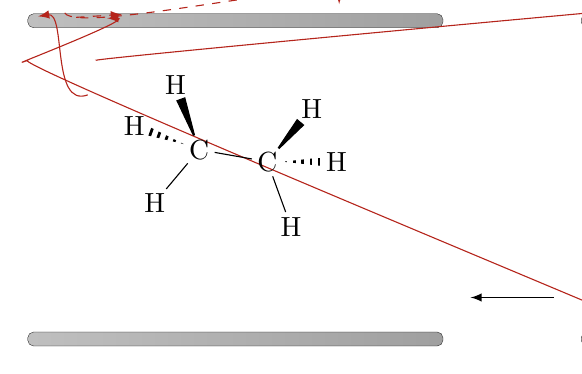
\begin{tikzpicture}
	\newcommand{\bondLength}{2.5em}
	\setchemfig{atom sep=\bondLength, cram width=0.3em}
	\newcommand{\blockHeight}{0.5em}
	\newcommand{\blockLength}{15em}
	\newcommand{\horizontalDistance}{5em}
	\newcommand{\arrowGap}{1em}
	\newcommand{\ethyleneHeight}{2*\bondLength}
	\newcommand{\hydrogenHeight}{\ethyleneHeight}
	\newcommand{\ethyleneRelativeX}{0.75}
	\newcommand{\hydrogenRelativeX}{0.25}
	\newcommand{\ethyleneAngle}{30}
	\newcommand{\verticalSpace}{\ethyleneHeight*1.5}
	\newcommand{\curvedArrowColor}{BrickRed}
	\newcommand{\arrowHeight}{\blockHeight + \bondLength/2}
	\newcommand{\ethyleneBondAngle}{120}

	%% First step
	\draw[left color = gray!50, right color = gray!75, line width = 0.01em, rounded corners = 0.2em] (0,0) rectangle (\blockLength,\blockHeight);

	\node[anchor=base] (ethylene) at (\blockLength*\ethyleneRelativeX,\ethyleneHeight+\blockHeight){\chemfig{[:{\ethyleneAngle}]C(<[::\ethyleneBondAngle]H)(<:[::360-\ethyleneBondAngle]H)=[@{doubleBond}]C(<:[::\ethyleneBondAngle-180]H)<[::180-\ethyleneBondAngle]H}};

	\node[anchor=base] at (\blockLength*\hydrogenRelativeX,\hydrogenHeight+\blockHeight){\chemfig{H-[@{hydrogenBond}]H}};

	\chemmove{
	\node (ethyleneAttackPoint) at (\blockLength*\ethyleneRelativeX,\blockHeight){};
	\node (hydrogenAttackPoint) at (\blockLength*\hydrogenRelativeX,\blockHeight){};
	\draw[shorten <= 0.5em,dashed,-latex,\curvedArrowColor] (doubleBond) .. controls +({-90+\ethyleneAngle}:5mm) and +(90:5mm).. (ethyleneAttackPoint);
	\draw[shorten <= 0.5em,dashed,-latex,\curvedArrowColor](hydrogenBond) -- (hydrogenAttackPoint);
	}

	\draw[->,-latex] (\blockLength + \arrowGap,\blockHeight+\bondLength/2) -- (\blockLength + \horizontalDistance -\arrowGap,\arrowHeight);

	%% 2nd step

	\draw[left color = gray!50, right color = gray!75,line width = 0.01em, rounded corners=0.2em] (\blockLength+\horizontalDistance,0) rectangle (\blockLength*2+\horizontalDistance,\blockHeight);

	\node[anchor=base] at (\blockLength*\ethyleneRelativeX + \blockLength + \horizontalDistance, \blockHeight + \bondLength - 3.5pt){\chemfig{C(<[::120]H)(<:[::170]H)(-[@{carbonSurfaceBond}::-90])-C(<:[::10]H)(<[::60]H)-[::-90]}};

	\node[anchor=base] at (\blockLength*\hydrogenRelativeX + \blockLength + \horizontalDistance,\blockHeight + \bondLength - 3.5pt){\chemfig{H(-[::-90])-[,,,,draw=none]@{hydrogenCaptured}H(-[@{hydrogenSurfaceBond}::-90])}};

	\chemmove{
	\node (surfaceSpot) at (\blockLength*\hydrogenRelativeX + \bondLength/2 + \blockLength + \horizontalDistance,\blockHeight) {};
	\draw[-latex,\curvedArrowColor] (carbonSurfaceBond) .. controls +(200:5mm) and +(0:5mm).. (hydrogenCaptured);
	\draw[-latex,\curvedArrowColor] (hydrogenSurfaceBond) .. controls +(180:3mm) and +(150:3mm).. (surfaceSpot);
	}

	\draw[->,-latex] (\blockLength + \horizontalDistance + \blockLength/2, -\arrowGap) -- (\blockLength + \horizontalDistance + \blockLength/2, -\horizontalDistance + \arrowGap);

	%% 3rd step

	\draw[left color = gray!50, right color = gray!75,line width = 0.01em, rounded corners=0.2em] (\blockLength+\horizontalDistance,-\horizontalDistance+\arrowGap-\verticalSpace) rectangle (\blockLength*2+\horizontalDistance,\blockHeight-\horizontalDistance+\arrowGap-\verticalSpace);

	\node[anchor=south] at (\blockLength*\ethyleneRelativeX + \blockLength + \horizontalDistance, \blockHeight - 3.5pt -\horizontalDistance+\arrowGap-\verticalSpace){\chemfig{[:-30]C(<[::120]H)(<:[::170]H)(-[::240]H)-C(<:[::10]H)(<[::60]H)-[@{secondCarbonSurfaceBond}:-90]}};

	\node[anchor=base] at (\blockLength*\hydrogenRelativeX + \blockLength + \horizontalDistance,\blockHeight + \bondLength - 3.5pt -\horizontalDistance+\arrowGap-\verticalSpace){\chemfig{@{secondHydrogenCaptured}H(-[@{secondHydrogenSurfaceBond}::-90])-[,,,,draw=none]}};

	\chemmove{
	\node (secondSurfaceSpot) at (\blockLength*\hydrogenRelativeX - \bondLength/2 + \blockLength + \horizontalDistance,\blockHeight-\horizontalDistance+\arrowGap-\verticalSpace) {};
	\draw[-latex,\curvedArrowColor] (secondCarbonSurfaceBond) .. controls +(200:5mm) and +(10:5mm).. (secondHydrogenCaptured);
	\draw[-latex,\curvedArrowColor] (secondHydrogenSurfaceBond) .. controls +(180:3mm) and +(150:4mm).. (secondSurfaceSpot);
	}

	\draw[->,-latex] (\blockLength + \horizontalDistance -\arrowGap,\arrowHeight-\horizontalDistance+\arrowGap-\verticalSpace) -- (\blockLength + \arrowGap,\blockHeight+\bondLength/2-\horizontalDistance+\arrowGap-\verticalSpace);

	%% 4rth step

	\draw[left color = gray!50, right color = gray!75, line width = 0.01em, rounded corners = 0.2em] (0,-\horizontalDistance+\arrowGap-\verticalSpace) rectangle (\blockLength,\blockHeight-\horizontalDistance+\arrowGap-\verticalSpace);

	\node[anchor=base] (ethane) at (\blockLength*.5,\ethyleneHeight*1.25+\blockHeight-\horizontalDistance+\arrowGap-\verticalSpace){\chemfig{[:-10]C(<[::120]H)(<:[::170]H)(-[::240]H)-C(<:[::10]H)(<[::60]H)-[::-60]H}};

\end{tikzpicture}
\end{figure}

\end{document}
